\documentclass[../monografia.tex]{subfiles}

\begin{document}

\chapter{BOM}
\begin{figure}[h]
\centering
    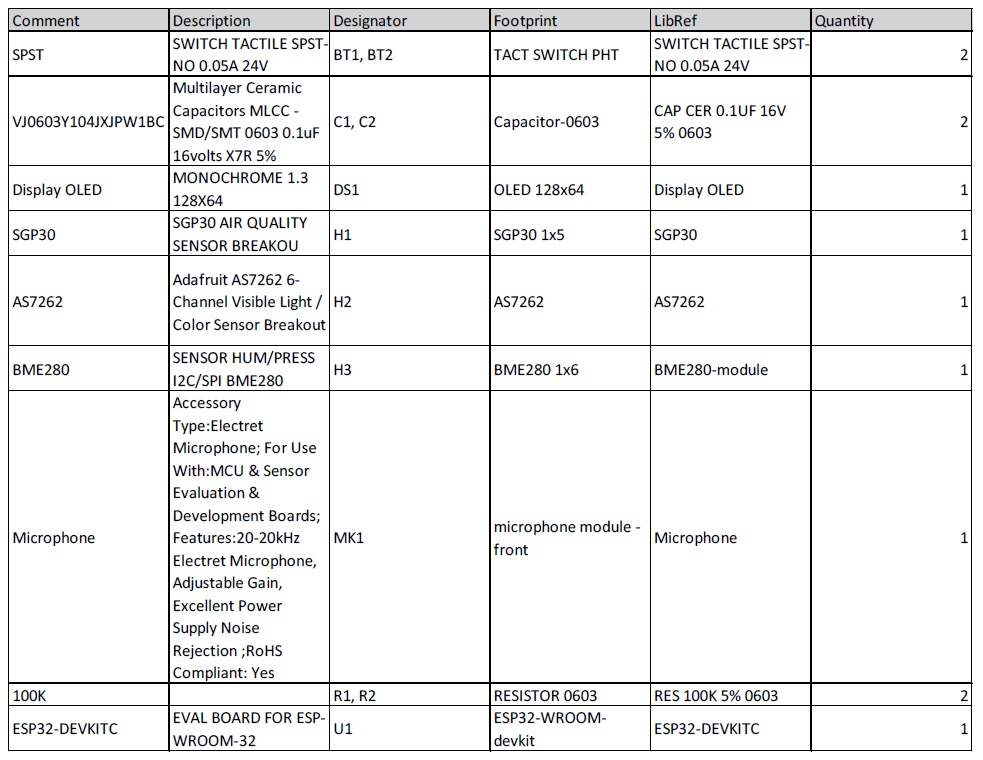
\includegraphics[width=.9\textwidth]{bom}
    \label{fig:img1}
    \caption{Bill of Materials (Lista de Materiais)}
\end{figure}

\chapter{Planejamento}

\begin{figure}[h]
    \centering
        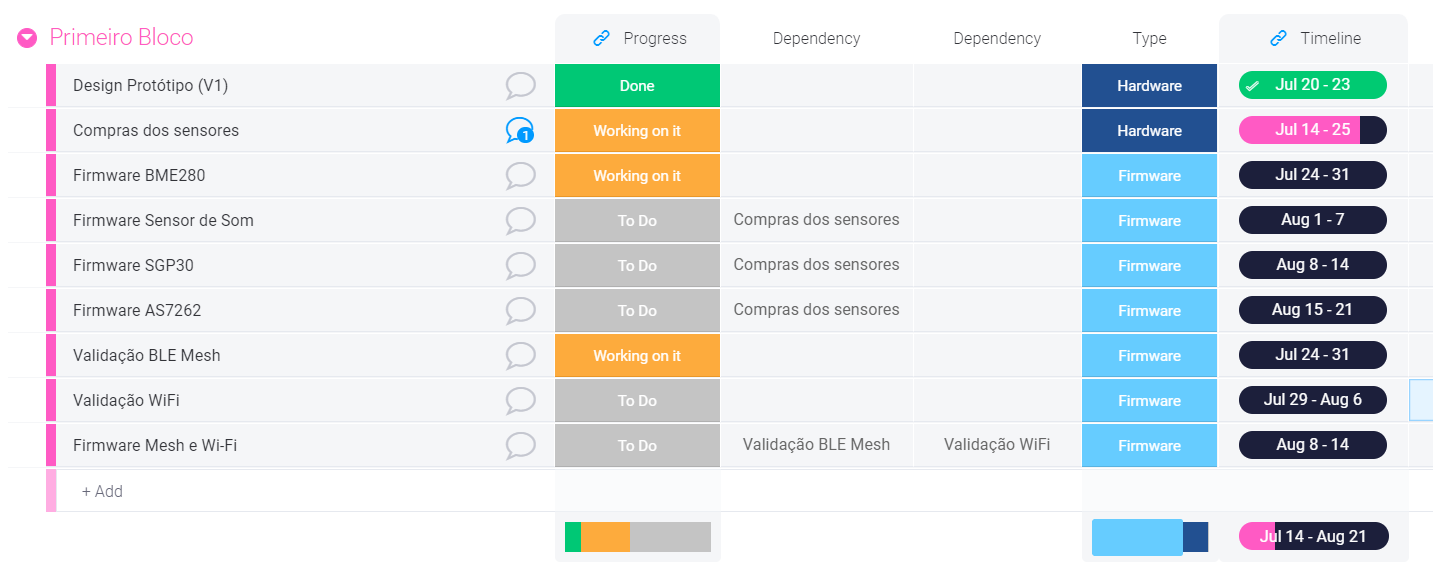
\includegraphics[width=.9\textwidth]{cronograma_b1}
        \label{fig:b1}
        \caption{Tarefas do Bloco 1}
\end{figure}
\begin{figure}[h]
    \centering
        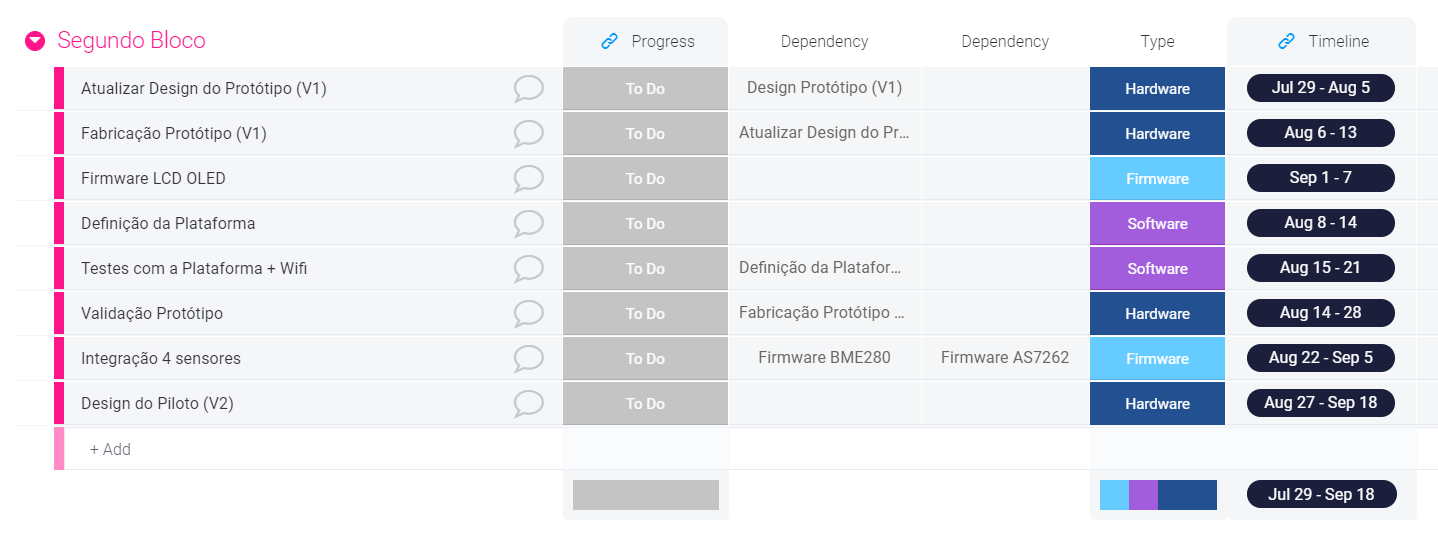
\includegraphics[width=.9\textwidth]{cronograma_b2}
        \label{fig:b2}
        \caption{Tarefas do Bloco 2}
\end{figure}
\begin{figure}[h]
    \centering
        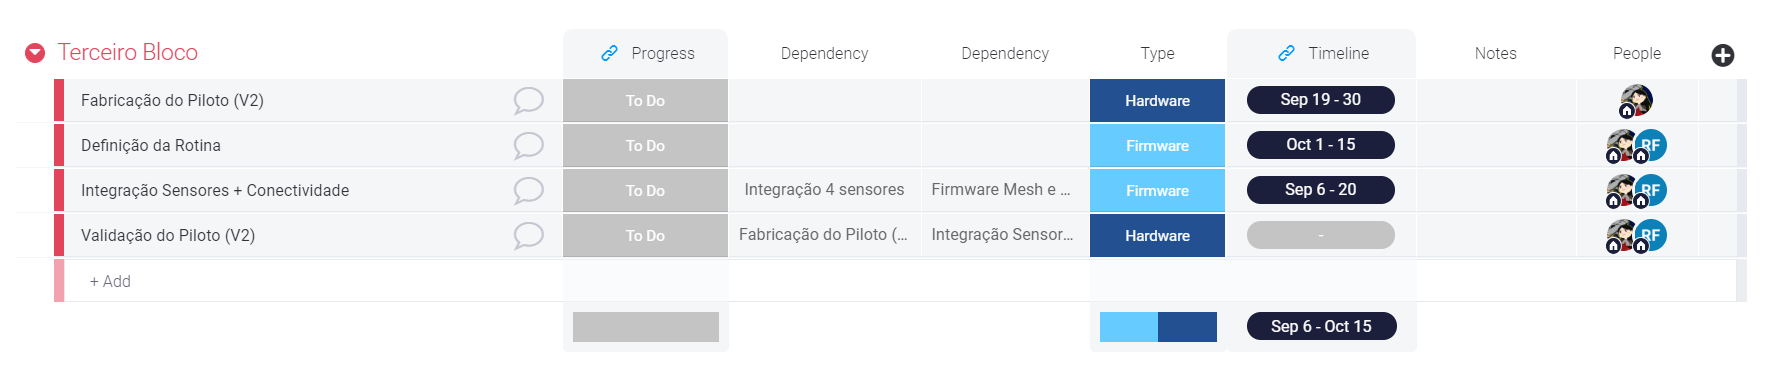
\includegraphics[width=.9\textwidth]{cronograma_b3}
        \label{fig:b3}
        \caption{Tarefas do Bloco 3}
\end{figure}

\chapter{Cronograma}

\begin{figure}[h]
    \centering
        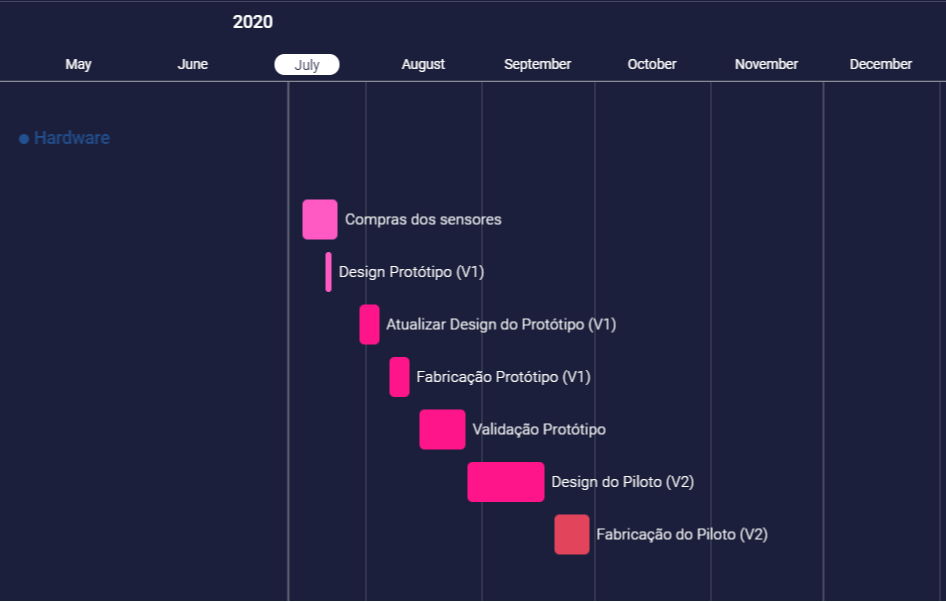
\includegraphics[width=.9\textwidth]{timeline_hw}
        \label{fig:hw}
        \caption{Cronograma de tarefas de hardware}
\end{figure}

\begin{figure}[h]
    \centering
        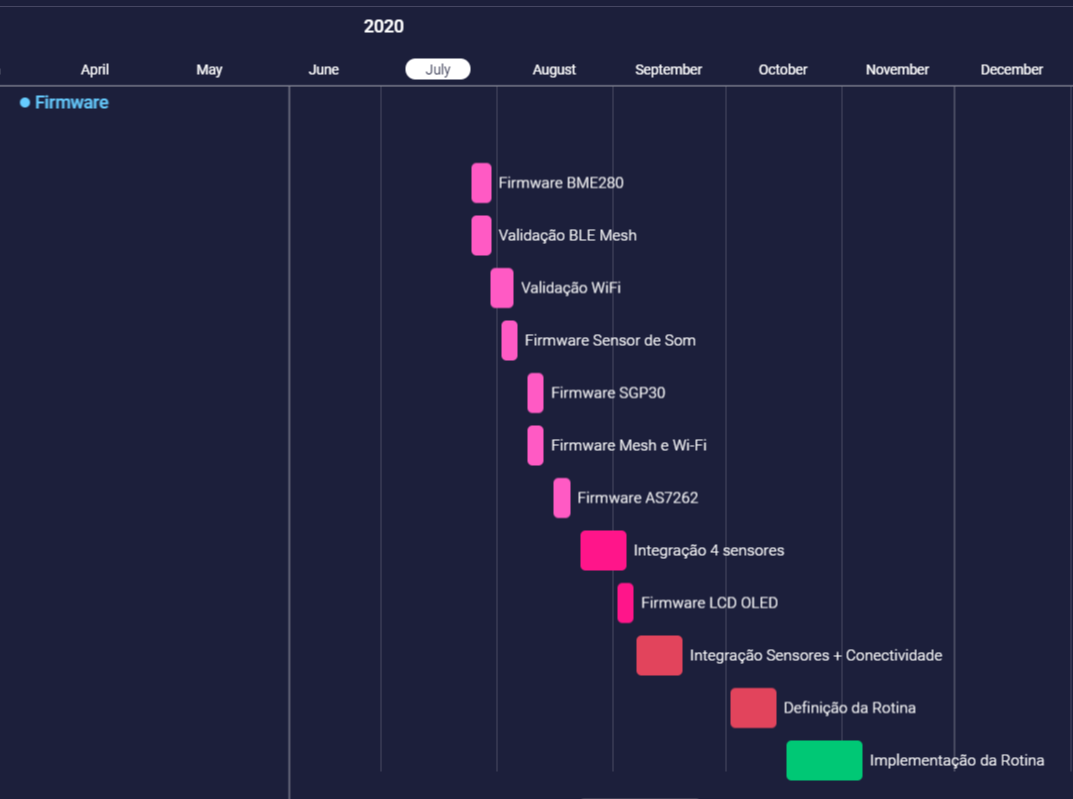
\includegraphics[width=.9\textwidth]{timeline_fw}
        \label{fig:fw}
        \caption{Cronograma de tarefas de firmware}
\end{figure}

\begin{figure}[h]
    \centering
        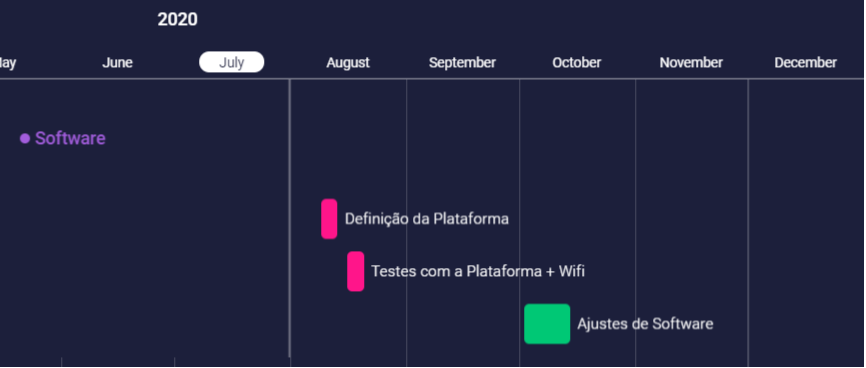
\includegraphics[width=.9\textwidth]{timeline_sw}
        \label{fig:sw}
        \caption{Cronograma de tarefas de software}
\end{figure}

\end{document}